\section{Methodology: Training a Robust Reward Model}
\label{sec:methodology}

The \carma{} framework trains robust reward models using a causally-motivated data augmentation strategy, outlined in Figure \ref{fig:data_augmentation_pipeline}. This involves two main phases: (1) generating attribute-aware counterfactual data based on our causal model (Section \ref{sec:preliminaries}), and (2) training the reward model $\hat{\mathrm{R}}_\theta$ with a specialized loss on the combined data.


\subsection{Attribute-Aware Counterfactual Data Generation}
\label{subsec:data_generation_phase}

This phase prepares the augmented dataset $\mathcal{D}_{\mathrm{aug}} = \mathcal{D}_{\mathrm{causal}} \cup \mathcal{D}_{\mathrm{neutral}}$ required for robust training, involving three conceptual steps:

\paragraph{Step 1: Attribute Identification.}
As a prerequisite, we identify the Principal Causal Components $\mathrm{C} = (\mathrm{C}_1, \dots, \mathrm{C}_\ell)$ relevant to the task, leveraging the causal framework from Section \ref{subsec:causal_graph}. This typically involves LLM prompting and refinement (Details in Appendix~\ref{subsec:attribute_identification_appendix}).

\begin{figure}[t!]
\centering
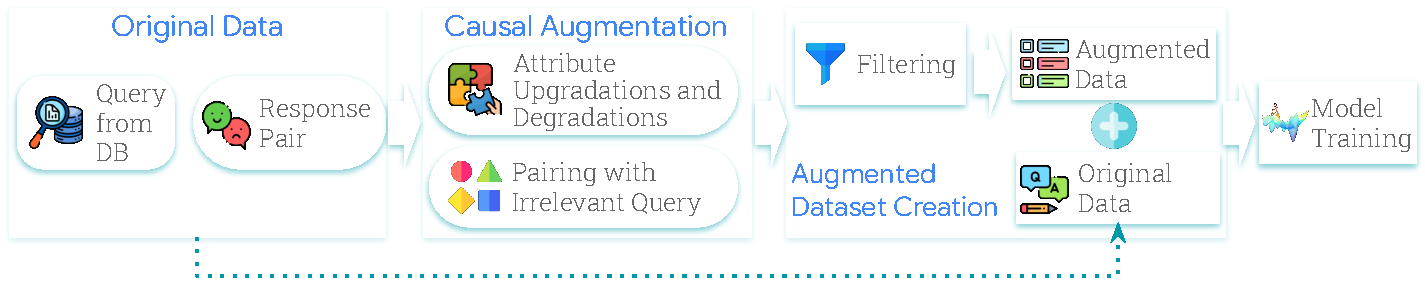
\includegraphics[width=\linewidth]{images/DataAugmentationPipeline.pdf} % Assuming this path is correct
\caption{The \carma{} data augmentation pipeline. Original preference data ($\mathcal{D}_{\mathrm{pref}}$) is used as a basis to generate: (1) \textit{Causal Augmentations} ($\mathcal{D}_{\mathrm{causal}}$) by performing \textbf{Attribute Upgradation and Degradation} on specific attributes to enforce sensitivity to genuine quality drivers, and (2) \textit{Neutral Augmentations} ($\mathcal{D}_{\mathrm{neutral}}$) via Irrelevant Query Neutrals (with tie-labels) to teach spurious feature 
invariance. After optional filtering, the reward model is trained on the combined original and augmented dataset.}
\label{fig:data_augmentation_pipeline}
\end{figure}

\paragraph{Step 2: Counterfactual Generation.}
Using the identified attributes $\mathrm{C}$, we generate synthetic data pairs via LLM-approximated counterfactuals, as defined in Section \ref{subsec:approximating_counterfactuals}. Following the strategies summarized in Table \ref{tab:augmentation_summary} and detailed conceptually in Section \ref{subsec:data_augmentation}, we create:
\vspace{-0.1in}
\begin{itemize}[itemsep=0pt, left=10pt]
    \item \textit{Causal Augmentation Pairs} ($\mathcal{D}_{\mathrm{causal}}$): Examples enforcing sensitivity to individual causal attributes $\mathrm{C}_j$ via \textbf{Attribute Upgradation} and \textbf{Degradation}, with  standard preference labels ($\succ$).
    \item \textit{Neutral Augmentation Pairs} ($\mathcal{D}_{\mathrm{neutral}}$): Examples enforcing invariance to spurious attributes $\mathrm{SP}$ while ensuring $\mathrm{C}$ is irrelevant or holding causal content $\mathrm{C}$ constant.   These are generated via \textbf{Irrelevant Query Neutrals} and \textbf{Causally Aligned Neutrals} respectively. These receive tie labels ($\approx$).
\end{itemize}
LLM prompts are in Appendix~\ref{sec:prompt_templates}. This yields the raw $\mathcal{D}_{\mathrm{aug}}$.

\vspace{-0.1in}
\paragraph{3. Data Filtering.} $\mathcal{D}_{\mathrm{aug}}$ is filtered to $\mathcal{D}_{\mathrm{aug\_filtered}}$ by retaining pairs where a baseline RM (trained on $\mathcal{D}_{\mathrm{pref}}$) is uncertain or incorrect, focusing training on informative examples (details: Section \ref{sec:experiments}, Appendix \ref{subsec:filtering_appendix}). This yields the final training datasets $\mathcal{D}_{\mathrm{pref}}$ and $\mathcal{D}_{\mathrm{aug\_filtered}}$.

% \vspace{-0.1in}
\subsection{Robust Reward Model Training}
\label{subsec:training_phase}

% \vspace{-0.05in}
Given the original data $\mathcal{D}_{\mathrm{pref}}$ and the filtered augmented data $\mathcal{D}_{\mathrm{aug\_filtered}}$, the final \carma{} reward model $\hat{\mathrm{R}}_\theta$ is trained by minimizing a composite loss function $\mathcal{L}(\theta)$ over the combined dataset $\mathcal{D} = \mathcal{D}_{\mathrm{pref}} \cup \mathcal{D}_{\mathrm{aug\_filtered}}$:


\begin{equation}
\mathcal{L}(\theta)=
-\underbrace{%
  \sum_{\substack{(\mathrm{Q},\mathrm{y}_w,\mathrm{y}_l)\\
                 \in\,\mathcal{D}_{\mathrm{pref}}\cup\mathcal{D}_{\mathrm{causal}}}}
  \!\log\!\bigl[\sigmoid(\Delta_{wl})\bigr]}_{\text{Preference Loss (Causal Sensitivity)}}
-\lambda\,\underbrace{%
  \sum_{\substack{(\mathrm{Q},\mathrm{A}_1,\mathrm{A}_2,\,y=\text{tie})\\
                 \in\,\mathcal{D}_{\mathrm{neutral}}}}
  \!\left(-\frac{1}{2}\bigl[\log\sigmoid(\Delta_{12})+\log\sigmoid(-\Delta_{12})\bigr]\right)}_{\text{Neutral Tie Loss (Spurious Invariance)}}
\label{eq:combined_loss_methodology}
\end{equation}


where $\Delta_{wl} = \hat{\mathrm{R}}_\theta(\mathrm{Q}, \mathrm{A}_w) - \hat{\mathrm{R}}_\theta(\mathrm{Q}, \mathrm{A}_l)$ and $\Delta_{12} = \hat{\mathrm{R}}_\theta(\mathrm{Q}, \mathrm{A}_1) - \hat{\mathrm{R}}_\theta(\mathrm{Q}, \mathrm{A}_2)$. The first term (Preference Loss) trains sensitivity to causal quality using $\mathcal{D}_{\mathrm{pref}}$ and $\mathcal{D}_{\mathrm{causal}}$. The second term (Neutral Tie Loss, weighted by $\lambda \ge 0$) trains invariance to spurious features using $\mathcal{D}_{\mathrm{neutral}}$ by encouraging $\Delta_{12} \approx 0$ for tie-labeled pairs. For our current set of experiments we keep $\lambda = 1$.

This optimization guides $\hat{\mathrm{R}}_\theta$ to be sensitive to causal attributes $\mathrm{C}$ while remaining robust to variations in spurious attributes $\mathrm{SP}$. We demonstrate \carma{}'s effectiveness in mitigating reward hacking and improving downstream policy performance in Section \ref{sec:experiments}.